\chapter{Derivatives}
\label{app:derivatives}

\section{Derivative of Cross Product}
\label{sec:app_d_cross_product}
The derivative of a cross product can be calculated analogue to matrix derivatives.
The skew symmetric cross matrix is
\begin{equation}
\mathbf{a}^\times = \left[
\begin{array}{ccc}
0 & -a_3 & a_2 \\
a_3 & 0 & -a_1 \\
-a_2 & a_1 & 0
\end{array} \right]
\end{equation}
and the appropriate derivatives are therefore
\begin{equation}
\frac{\partial}{\partial \mathbf{a}} \left( \mathbf{a} \times \mathbf{b} \right)
= - \mathbf{b}^\times
\end{equation}
and
\begin{equation}
\frac{\partial}{\partial \mathbf{a}} \left( \mathbf{b} \times \mathbf{a} \right)
=  \mathbf{b}^\times
\end{equation}

\section{Derivative w.r.t. Gibbs-Rodriquez Parameters}
\label{sec:app_dwrt_rodriquez}
Derivative of the rotation matrix \cref{eq:rod_to_C} w.r.t. the Gibbs-Rodriquez parameter:

\begin{equation*}
\frac{\partial \mathbf{C}}{\partial \lambda_1} = 
\left(\begin{array}{ccc} 
\frac{4\, {\lambda_1}\, \left({{\lambda_2}}^2 + {{\lambda_3}}^2\right)}{\nu}^2 & 
\frac{2\, {\lambda_2}}{\nu} + \frac{4\, {\lambda_1}\, {\lambda_3} - {\lambda_1}\, {\lambda_2}}{\nu^2} & 
\frac{2\, {\lambda_3}}{\nu} - \frac{4\, {\lambda_1}\, \left({\lambda_2} + {\lambda_1}\, {\lambda_3}\right)}{\nu^2}\\ 
\frac{2\, {\lambda_2}}{\nu} - \frac{4\, {\lambda_1}\, \left({\lambda_3} + {\lambda_1}\, {\lambda_2}\right)}{\nu^2} & 
\frac{4\, {\lambda_1}\, \left({{\lambda_1}}^2 + {{\lambda_3}}^2\right)}{\nu^2} - \frac{4\, {\lambda_1}}{\nu} &
\frac{4\, {\lambda_1}\, \left({\lambda_1} - {\lambda_2}\, {\lambda_3}\right)}{\nu^2} - \frac{2}{\nu}\\
\frac{2\, {\lambda_3}}{\nu} + \frac{4\, {\lambda_1}\, \left({\lambda_2} - {\lambda_1}\, {\lambda_3}\right)}{\nu^2} &
\frac{2}{\nu} - \frac{4\, {\lambda_1}\, \left({\lambda_1} + {\lambda_2}\, {\lambda_3}\right)}{\nu^2} & \frac{4\, {\lambda_1}\, \left({{\lambda_1}}^2 + {{\lambda_2}}^2\right)}{\nu^2} - \frac{4\, {\lambda_1}}{\nu}
\end{array}\right)
\end{equation*}

\begin{equation*}
\frac{\partial \mathbf{C}}{\partial \lambda_2} = 
\left(\begin{array}{ccc} 
\frac{4\, {\lambda_2}\, \left({{\lambda_2}}^2 + {{\lambda_3}}^2\right)}{{\nu}^2} - \frac{4\, {\lambda_2}}{\nu} &
\frac{2\, {\lambda_1}}{\nu} + \frac{4\, {\lambda_2}\, \left({\lambda_3} - {\lambda_1}\, {\lambda_2}\right)}{{\nu}^2} &
\frac{2}{\nu} - \frac{4\, {\lambda_2}\, \left({\lambda_2} + {\lambda_1}\, {\lambda_3}\right)}{{\nu}^2}\\
\frac{2\, {\lambda_1}}{\nu} - \frac{4\, {\lambda_2}\, \left({\lambda_3} + {\lambda_1}\, {\lambda_2}\right)}{{\nu}^2} &
\frac{4\, {\lambda_2}\, \left({{\lambda_1}}^2 + {{\lambda_3}}^2\right)}{{\nu}^2} & \frac{2\, {\lambda_3}}{\nu} + \frac{4\, {\lambda_2}\, \left({\lambda_1} - {\lambda_2}\, {\lambda_3}\right)}{{\nu}^2}\\
\frac{4\, {\lambda_2}\, \left({\lambda_2} - {\lambda_1}\, {\lambda_3}\right)}{{\nu}^2} - \frac{2}{\nu} &
\frac{2\, {\lambda_3}}{\nu} - \frac{4\, {\lambda_2}\, \left({\lambda_1} + {\lambda_2}\, {\lambda_3}\right)}{{\nu}^2} &
\frac{4\, {\lambda_2}\, \left({{\lambda_1}}^2 + {{\lambda_2}}^2\right)}{{\nu}^2} - \frac{4\, {\lambda_2}}{\nu} \end{array}\right)
\end{equation*}

\begin{equation*}
\frac{\partial \mathbf{C}}{\partial \lambda_3} = 
\left(\begin{array}{ccc} \frac{4\, {\lambda_3}\, \left({{\lambda_2}}^2 + {{\lambda_3}}^2\right)}{{\nu}^2} - \frac{4\, {\lambda_3}}{\nu} & \frac{4\, {\lambda_3}\, \left({\lambda_3} - {\lambda_1}\, {\lambda_2}\right)}{{\nu}^2} - \frac{2}{\nu} & \frac{2\, {\lambda_1}}{\nu} - \frac{4\, {\lambda_3}\, \left({\lambda_2} + {\lambda_1}\, {\lambda_3}\right)}{{\nu}^2}\\ \frac{2}{\nu} - \frac{4\, {\lambda_3}\, \left({\lambda_3} + {\lambda_1}\, {\lambda_2}\right)}{{\nu}^2} & \frac{4\, {\lambda_3}\, \left({{\lambda_1}}^2 + {{\lambda_3}}^2\right)}{{\nu}^2} - \frac{4\, {\lambda_3}}{\nu} & \frac{2\, {\lambda_2}}{\nu} + \frac{4\, {\lambda_3}\, \left({\lambda_1} - {\lambda_2}\, {\lambda_3}\right)}{{\nu}^2}\\ \frac{2\, {\lambda_1}}{\nu} + \frac{4\, {\lambda_3}\, \left({\lambda_2} - {\lambda_1}\, {\lambda_3}\right)}{{\nu}^2} & \frac{2\, {\lambda_2}}{\nu} - \frac{4\, {\lambda_3}\, \left({\lambda_1} + {\lambda_2}\, {\lambda_3}\right)}{{\nu}^2} & \frac{4\, {\lambda_3}\, \left({{\lambda_1}}^2 + {{\lambda_2}}^2\right)}{{\nu}^2} \end{array}\right)
\end{equation*}
where
\begin{equation*}
\nu = {\lambda_1}^2 + {\lambda_2}^2 + {\lambda_3}^2 + 1
\end{equation*}


%\section{Derivative w.r.t. Inertia Tensor A}
%XXX derivative w.r.t inertia tensor components (and it's inverse)

%\section{Derivative w.r.t. Inertia Tensor B}
%XXX derivative w.r.t diagonal inertia tensor and rotation matrix (and it's inverse)

\chapter{Additional Plots}

\section{Sensor Specification}
\begin{figure}[hbtp]
\captionsetup{width=0.9\textwidth}
\centering
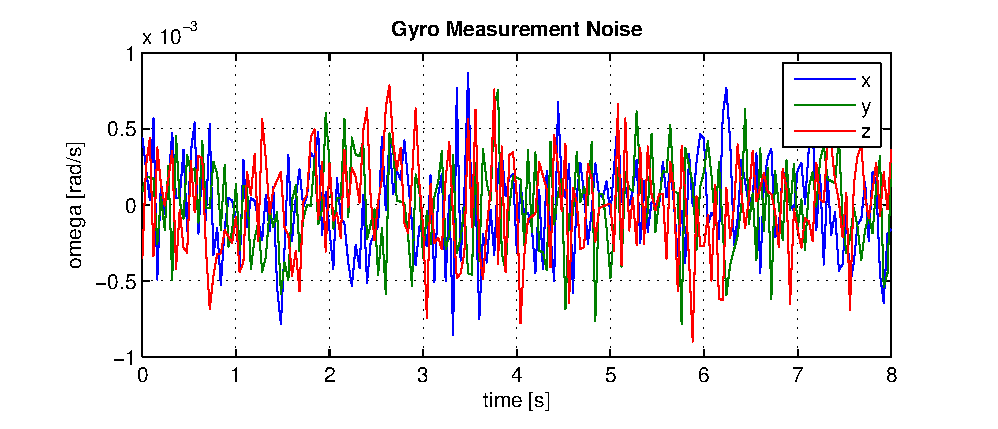
\includegraphics[width = \textwidth]{images/appendix/gyro_noise.eps}
\caption{Measurement noise of MPU-6000 gyro. The RMS error is about $3.2 \cdot 10^{-4} rad/s$.}
\label{fig:gyro_noise}

\end{figure}
\begin{figure}[hbtp]
\captionsetup{width=0.9\textwidth}
\centering
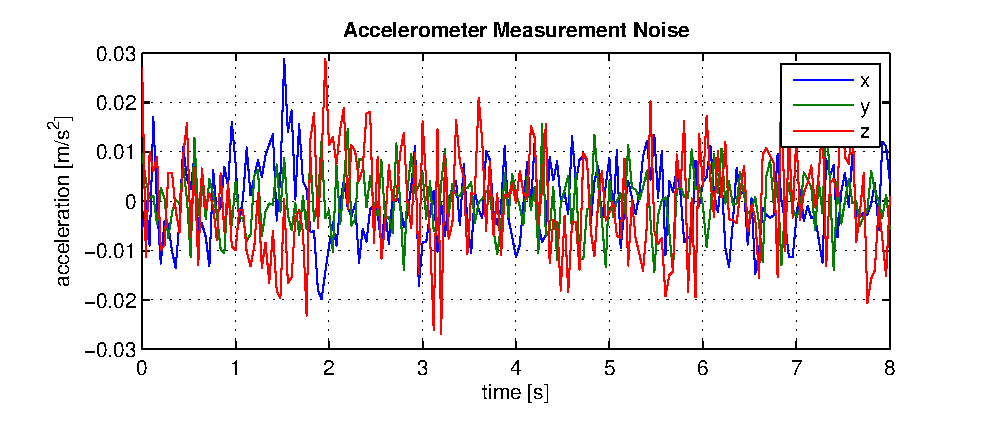
\includegraphics[width = \textwidth]{images/appendix/accel_noise.eps}
\caption{Measurement noise of MPU-6000 accelerometer. The RMS error is about $8.2 \cdot 10^{-3} m/s^2$.}
\label{fig:accel_noise}
\end{figure}



\section{Actuation Unit Position Estimate Variance}
\begin{figure}[hbtp]
\captionsetup{width=0.9\textwidth}
\centering
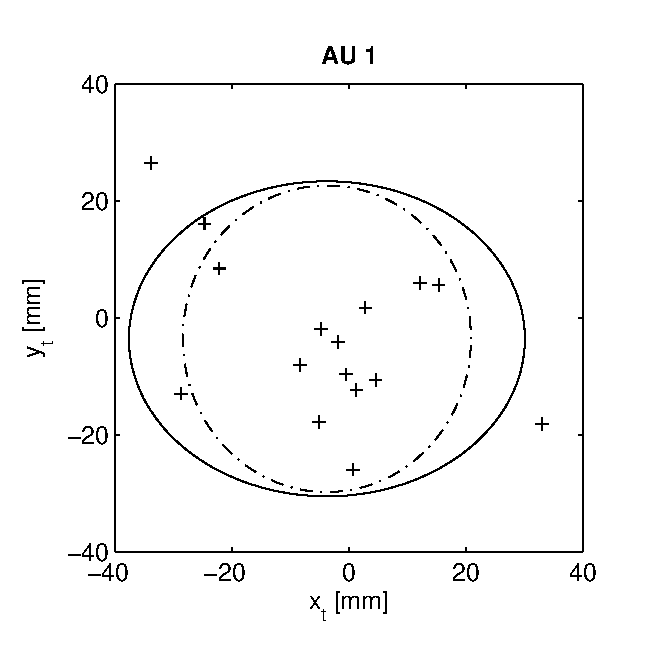
\includegraphics[width = 0.45\textwidth]{images/results/confidence_95_interval_AU1.eps}
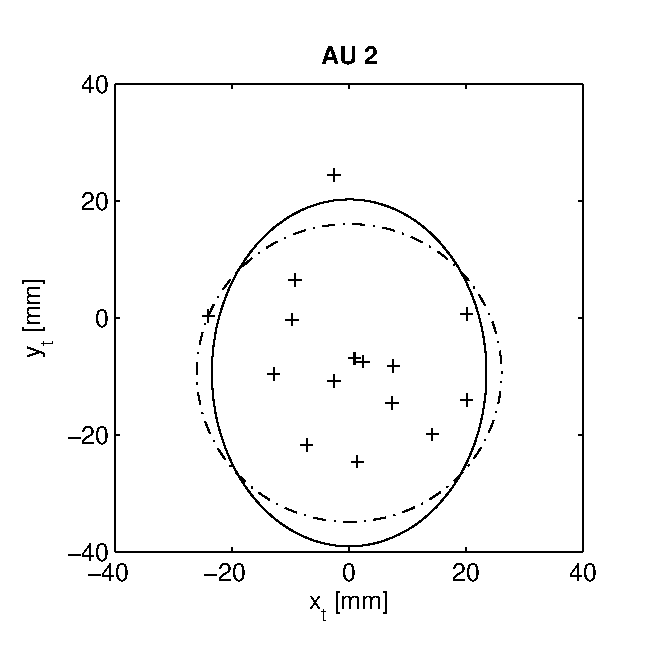
\includegraphics[width = 0.45\textwidth]{images/results/confidence_95_interval_AU2.eps} \\
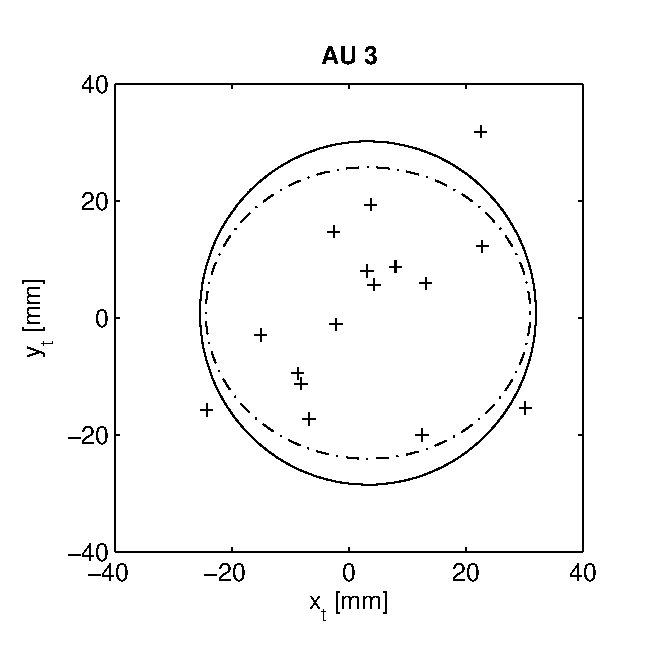
\includegraphics[width = 0.45\textwidth]{images/results/confidence_95_interval_AU3.eps}
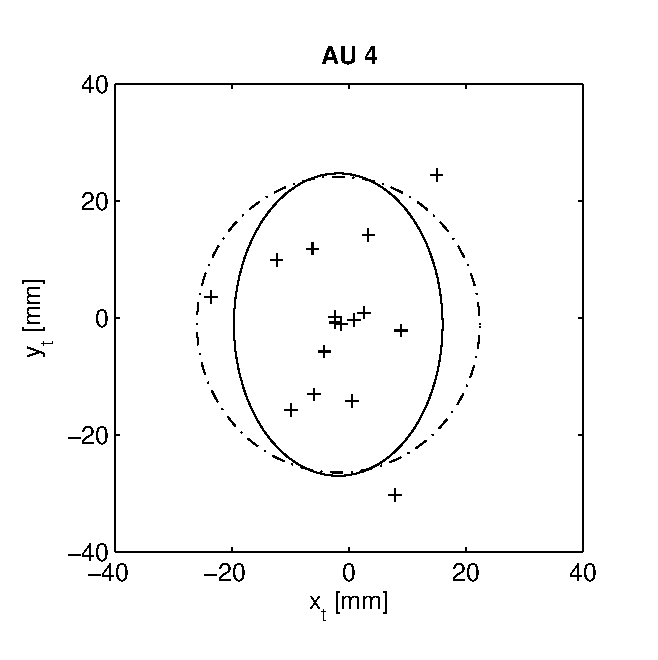
\includegraphics[width = 0.45\textwidth]{images/results/confidence_95_interval_AU4.eps}
\caption{Distribution of actuator position estimates. 16 datasets with 24 input vectors each and one sample per input vector.
$\mathbf{+}$ represent the results used to measure the variance.
\textbf{dashed}: 95\% confidence interval calculated from covariance matrix.
\textbf{solid}: 95\% confidence interval calculated from multiple results. }
\label{fig:result_95pc_confidence_all}
\end{figure}


\section{Parameter Estimates}
\label{sec:app_parameter_est}

\begin{table}[H]
\begin{tabular}{lcrrrc}
Variable & Parameter & Mean & Std1 & Std2 & Unit \\
\hline \hline
AU 1 Orientation & $\lambda_1^1$ & -1.742 & 0.0092 & 0.0125 & $[-]$ \\
                 & $\lambda_1^1$ & -0.177 & 0.0027 & 0.0050 & $[-]$ \\
                 & $\lambda_1^1$ &  0.306 & 0.0058 & 0.0058 & $[-]$ \\
AU 2 Orientation & $\lambda_1^2$ &  1.731 & 0.0092 & 0.0124 & $[-]$ \\
                 & $\lambda_1^2$ & -0.175 & 0.0044 & 0.0051 & $[-]$ \\
                 & $\lambda_1^2$ & -0.306 & 0.0053 & 0.0060 & $[-]$ \\
AU 3 Orientation & $\lambda_1^3$ &  0.001 & 0.0030 & 0.0030 & $[-]$ \\
                 & $\lambda_1^3$ & -0.177 & 0.0020 & 0.0034 & $[-]$ \\
                 & $\lambda_1^3$ &  0.000 & 0.0019 & 0.0022 & $[-]$ \\
AU 4 Orientation & $\lambda_1^3$ & -0.001 & 0.0018 & 0.0037 & $[-]$ \\
                 & $\lambda_1^3$ &  1.002 & 0.0038 & 0.0059 & $[-]$ \\
                 & $\lambda_1^3$ & -0.001 & 0.0018 & 0.0036 & $[-]$ \\
\hline
Inertia Tensor & $J_1$ & 14.574 & 0.0239 & 0.0361 & kg m$^2$ \\
               & $J_2$ & 15.564 & 0.0219 & 0.0379 & kg m$^2$ \\
               & $J_3$ & 15.475 & 0.0350 & 0.0391 & kg m$^2$ \\
               & $J_4$ &  0.072 & 0.0245 & 0.0210 & kg m$^2$ \\
               & $J_5$ &  0.215 & 0.0173 & 0.0203 & kg m$^2$ \\
               & $J_6$ &  0.047 & 0.0085 & 0.0199 & kg m$^2$ \\
\hline
Center of Gravity & $\mathbf{p}_{b,x}^{cob,cog}$ & -0.102 & 0.1114 & 0.1530 & mm \\
                  & $\mathbf{p}_{b,y}^{cob,cog}$ & -0.025 & 0.1502 & 0.1493 & mm \\
                  & $\mathbf{p}_{b,z}^{cob,cog}$ & -0.003 & 0.0990 & 0.1478 & mm \\
\hline
\end{tabular}
\caption{Optimization result of the parameters as defined in \cref{sec:parameterization}, \cref{tab:params_updated} for simulation data. Results have been calculated for 16 distinct datasets. \textbf{Mean} is the mean parameter estimate of the samples with standard deviation \textbf{Std1}. The mean over the expected standard deviation from the optimization residual is given as \textbf{Std2}.}
\end{table}

\begin{table}[H]
\begin{tabular}{lcrrrc}
Variable & Parameter & Mean & Std1 & Std2 & Unit \\
\hline \hline
AU 1 Orientation & $\lambda_1^1$ & -1.842 & 0.0390 & 0.0465 & $[-]$ \\
                 & $\lambda_2^1$ & -0.253 & 0.0134 & 0.0155 & $[-]$ \\
                 & $\lambda_3^1$ &  0.270 & 0.0161 & 0.0161 & $[-]$ \\
AU 2 Orientation & $\lambda_1^2$ &  1.727 & 0.0330 & 0.0414 & $[-]$ \\
                 & $\lambda_2^2$ & -0.018 & 0.0136 & 0.0125 & $[-]$ \\
                 & $\lambda_3^2$ & -0.335 & 0.0180 & 0.0212 & $[-]$ \\
AU 3 Orientation & $\lambda_1^3$ & -0.010 & 0.0079 & 0.0091 & $[-]$ \\
                 & $\lambda_2^3$ & -0.183 & 0.0093 & 0.0114 & $[-]$ \\
                 & $\lambda_3^3$ & -0.006 & 0.0054 & 0.0044 & $[-]$ \\
AU 4 Orientation & $\lambda_1^4$ & -0.104 & 0.0088 & 0.0097 & $[-]$ \\
                 & $\lambda_2^4$ &  0.985 & 0.0168 & 0.0209 & $[-]$ \\
                 & $\lambda_3^4$ & -0.097 & 0.0092 & 0.0107 & $[-]$ \\
\hline
Inertia Tensor & $J_1$ & 14.709 & 0.1356 & 0.2695 & kg m$^2$ \\
               & $J_2$ & 17.218 & 0.1759 & 0.3285 & kg m$^2$ \\
               & $J_3$ & 16.405 & 0.1685 & 0.4151 & kg m$^2$ \\
               & $J_4$ &  0.512 & 0.1351 & 0.1366 & kg m$^2$ \\
               & $J_5$ & -0.060 & 0.1261 & 0.1460 & kg m$^2$ \\
               & $J_6$ &  0.234 & 0.1267 & 0.1342 & kg m$^2$ \\
\hline
Center of Gravity & $\mathbf{p}_{b,x}^{cob,cog}$ &  0.495 & 0.2842 & 0.2695 & mm \\
                  & $\mathbf{p}_{b,y}^{cob,cog}$ & -0.706 & 0.2679 & 0.2285 & mm \\
                  & $\mathbf{p}_{b,z}^{cob,cog}$ & -0.215 & 0.3171 & 0.3384 & mm \\
\hline
\end{tabular}
\caption{Optimization result of the parameters as defined in \cref{sec:parameterization}, \cref{tab:params_updated} for real data. Results have been calculated for 16 distinct datasets. \textbf{Mean} is the mean parameter estimate of the samples with standard deviation \textbf{Std1}. The mean over the expected standard deviation from the optimization residual is given as \textbf{Std2}. }
\end{table}
